\chapter{Description of Fortune's algorithm}

We are now ready to describe Fortune's algorithm. We start with describing an overview of the algorithm, and then in the next section we describe some of the details thoroughly -- so anytime the algorithm says ``see detail $n$'', then this detail can be found in the next section.

\begin{alg} \label{alg:fortune} \textsc{VoronoiDiagram}(P) \\
\textit{Input:} A set $P = \curly{p_1, \ldots, p_n}$ of point sites in the plane. \\
\textit{Output:} The Voronoi diagram $\Vor(P)$ given inside a bounding box in a doubly-connected edge list $\mathcal{D}$.
\begin{enumerate}
    \item Initialize the event queue $\mathcal{Q}$ with a site event for every point in $P$, initialize the beach line tree $\mathcal{T}$ to be \textsc{nil}, and let the DCEL $\mathcal{D}$ be empty.
    \item Repeat the following until $\mathcal{Q}$ is empty:
    \begin{enumerate}[i.]
        \item Remove the event $e$ with the largest $y$-coordinate from $\mathcal{Q}$.
        \item If $e$ is a site event call \textsc{HandleSiteEvent}$(e)$.
        \item If $e$ is a site event call \textsc{HandleCircleEvent}$(e)$.
    \end{enumerate}
    \item At this point the internal nodes in $\mathcal{T}$ represent the infinite edges of $\Vor(P)$. Compute a bounding box $B$ which contains all points in $P$, as well as all the vertices of $\Vor(P)$, which are contained in $\mathcal{D}$. Intersect the infinite edges in $\mathcal{T}$ with $B$ and let these intersection points be new vertices in $\mathcal{D}$. Add new edges and pointers to make sure we still have a proper DCEL structure.
\end{enumerate}
\end{alg}

\begin{proc} \textsc{HandleSiteEvent}$(e)$
\begin{enumerate}
    \item Let $p_i$ denote the site that $e$ points to.
    \item If $\mathcal{T} = \textsc{nil}$ then let $\mathcal{T}$ store the single arc that is described by $p_i$ and return.
    \item Otherwise, $\mathcal{T} \ne \textsc{nil}$. Search in $\mathcal{T}$ for the arc $\alpha$ vertically above $p_i$, that is the arc at which the vertical line through $p_i$ intersects the beach line. (See detail \#)
    \item If $\alpha$ has a pointer to a circle event $e'$, then remove $e'$ from $\mathcal{Q}$, as this circle event is now a false alarm since $\alpha$ is about to disappear earlier than we initially thought.
    \item Create the new arc $\beta$ defined by $p_i$ and insert it into $\mathcal{T}$ as described in Section \ref{sec:insertingatsiteevents}. Update $\mathcal{D}$ by creating the new half-edges which will be traced out by the two new breakpoints as described in Section \ref{sec:dcelatsiteevents}.
    \item Check the triple of consecutive arcs where the new arc for $p_i$ is the left arc to see if the breakpoints converge. If so, insert the circle event into $\mathcal{Q}$ and add pointers between the node in $\mathcal{T}$ and the node in $\mathcal{Q}$. Do the same for the triple where the new arc is the right arc. (See detail \#)
\end{enumerate}
\end{proc}

\begin{proc} \textsc{HandleCircleEvent}$(e)$
\begin{enumerate}
    \item Let $\alpha$ be the arc pointed to by $e$, which is about to disappear from the beach line.
    \item Delete all circle events from $\mathcal{Q}$ which involve $\alpha$: The one where $\alpha$ is the middle arc has already been deleted, and the other two possible circle events where $\alpha$ is the left and right arc respectively can be found through $\alpha$'s \textsf{.leftArc} and \textsf{.rightArc} pointers. (See detail \#)
    \item Delete $\alpha$ from $\mathcal{T}$, how this is done is described in Section \ref{sec:deletingatsiteevents}.
    \item Add the center $c$ of the circle describing $e$ as a new vertex of $\mathcal{D}$. Connect the half-edges in $\mathcal{D}$ that converge at $e$, and create a new half-edge which starts at $c$ and setup the appropriate pointers. The details are given in Section \ref{sec:dcelatcircleevents}.
    \item As $\alpha$ disappears from the beach line, we get new triples of consecutive arcs which might have converging breakpoints that can lead to a circle event. Check these and add circle events if needed. (See detail \#)
\end{enumerate}
\end{proc}

\section{Details}

\subsection*{Detail 1: Intersecting lines}
As a subroutine in several steps during the algorithm we will need to intersect line segments or rays with each other. We start by describing a solution to this in general. This detail assumes that the reader is familiar with basic linear algebra. We want to find the intersection between 2 lines. We parametrize the lines as follows:
\[
    \gamma_1(t) = p + t d_1 \quad \text{and} \quad
    \gamma_2(s) = q + s d_2,
\]
where $p$ and $q$ are points on the lines, and $d_1$ and $d_2$ are direction vectors which tells us which way the lines point. The situation is illustrated as follows:
\[
    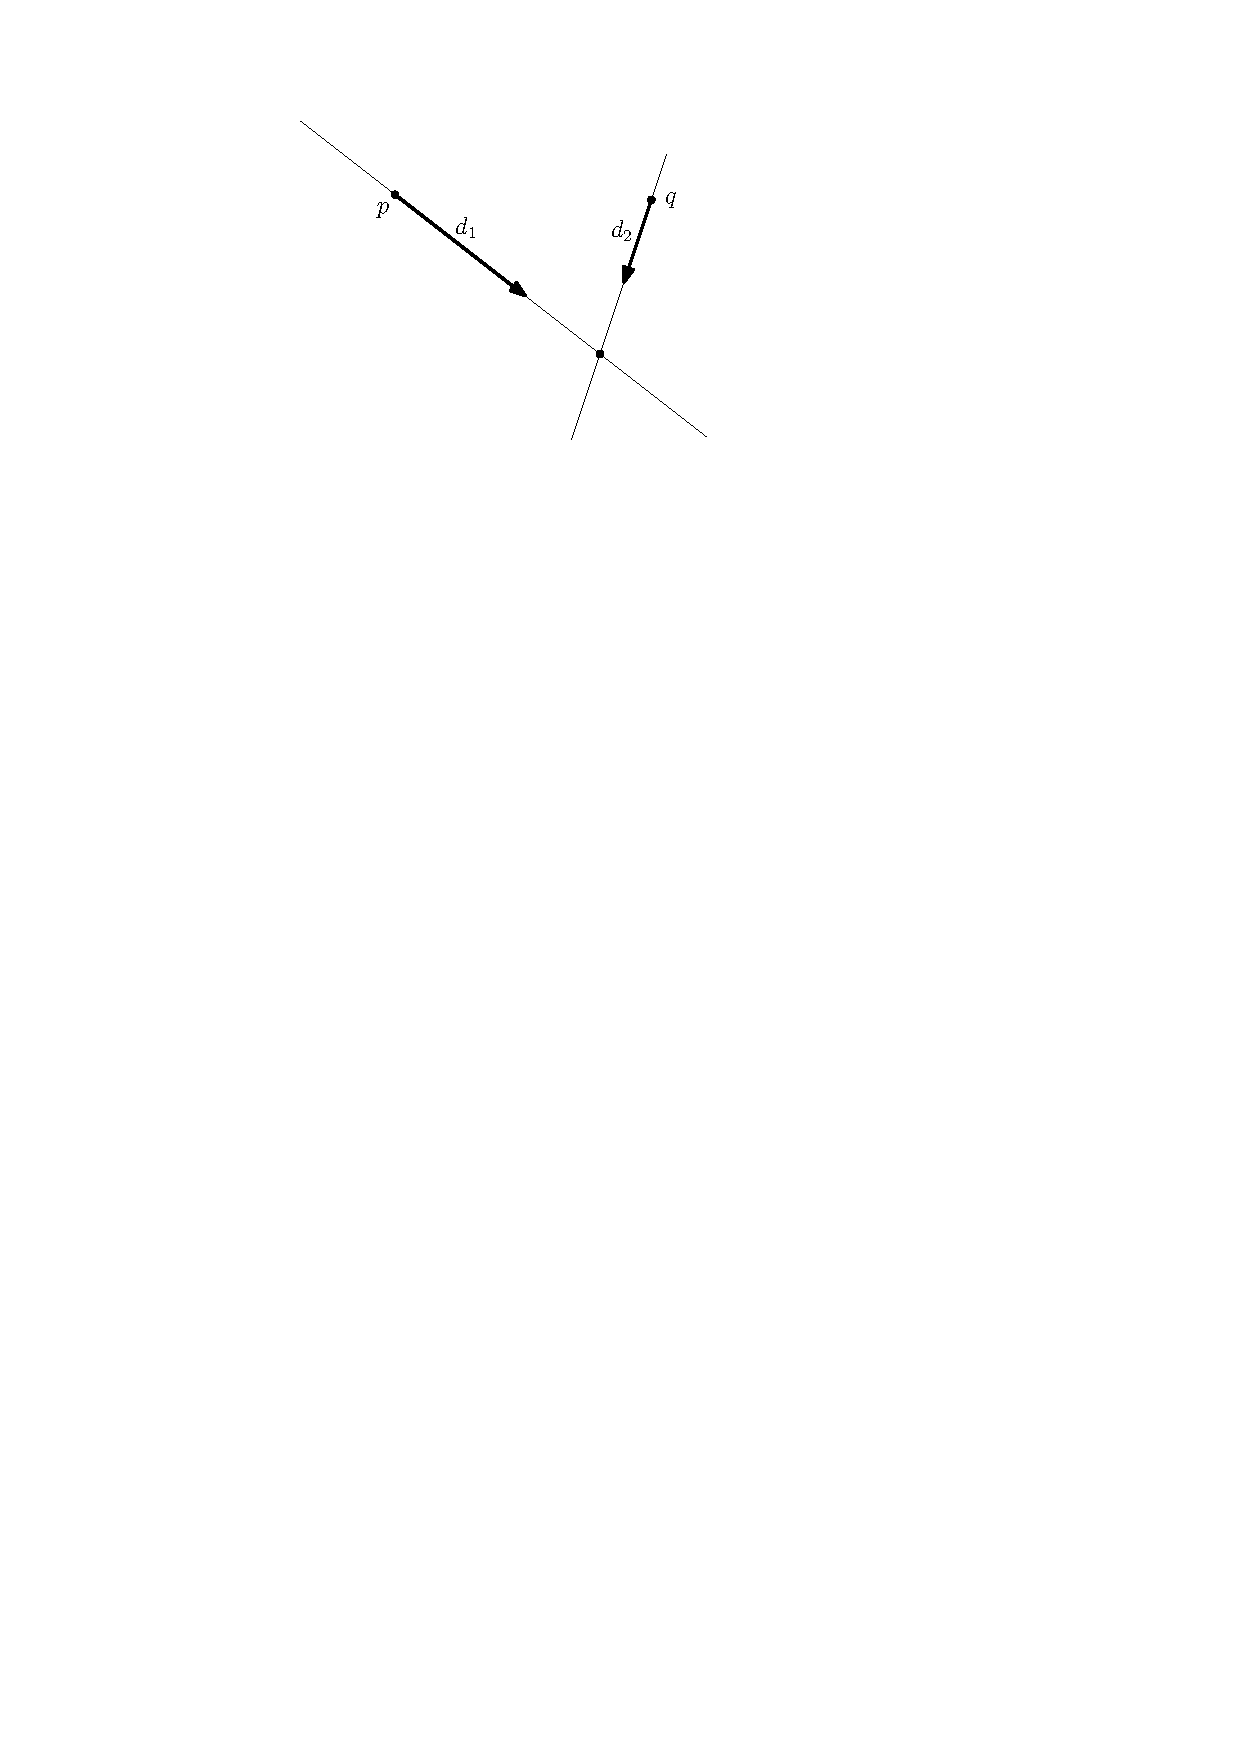
\includegraphics[scale=0.8]{intersect_lines}
\]
To find an intersection point, we must find $s, t \in \R$ such that
\[
    \gamma_1(t) = \gamma_2(s).
\]
That is, we want to solve
\[
    p + t d_1 = q + s d_2.
\]
This can be rewritten into the matrix equation
\[
    A \begin{pmatrix}
        s \\
        -t
    \end{pmatrix}
    =
    q - p,
\]
where $A = \begin{pmatrix} \mid & \mid \\ d_1 & d_2 \\ \mid & \mid \end{pmatrix}$ is the $2 \times 2$ matrix which has $d_1$ and $d_2$ as left and right columns, respectively. The equation system has a unique solution if $d_1$ and $d_2$ are linearly independent, and if they are, the solution is given by
\[
    \begin{pmatrix}
        s \\
        -t
    \end{pmatrix}
    =
    A^{-1} (q - p).
\]
This linear independence property is equivalent to checking that the determinant $\det(A)$ is non-zero. So, in order to check if two lines intersect, we first check if $\det(A) \ne 0$. If not, we say the lines don't intersect. Otherwise, they intersect, and we use the above solution to find the intersection point.

Now in the case of line segments and rays, we also need some constraints on $s$ and $t$, it is not enough that the lines themselves intersect.

To intersect line segments, where the first line segment is given as the points between $p_1$ and $p_2$, and the second line segment is given as the points between $q_1$ and $q_2$, then we let $p = p_1$ and $q = q_1$ and then set $d_1 = p_2 - p_1$ and $d_2 = q_2 - q_1$ and then we solve the equation system as above. If there is a solution to the equation system, then we also need to check that $s \in [0, 1]$ and $t \in [0, 1]$ in order for the intersection point to lie on both of the line segments.

Finally, we look at intersecting two rays. We describe the rays as the lines at the start of this detail, but now we have the requirement that $s, t \geq 0$, which gives us that the rays start at $p$ and $q$, and then they shoot out in the direction of $d_1$ and $d_2$, respectively.

\subsection*{Detail 2: Choose breakpoint based on the ordering of tuple}
Let $p_i$ and $p_j$ be two sites and let $\beta_i$ and $\beta_j$ be the hyperbolas that they describe. If a breakpoint stores the tuple $(p_i, p_j)$ then we want a way to find the $x$ coordinate of that breakpoint. Since the intersection of two hyperbolas may contain 2 intersection points, we need to pick the correct one. We already described this when discussing internal tree nodes at the start of Section \ref{sec:bst}, but let's recap: The order is important since the intersection of the hyperbolas defined by $p_i$ and $p_j$ consists of two points, and the order lets us tell these breakpoints apart. If we consider the beach line as running from the left to the right, then at every breakpoint an arc is leaving, and another is entering it. Thus the tuple $(p_i, p_j)$ tells us that we are interested in the breakpoint at which an arc pointing to $p_i$ leaves, and an arc pointing to $p_j$ is entering the beach line. We will need the following result:

\begin{prop} \label{prop:highschool1}
Let $f(x) = a x^2 + b x + c$ be a polynomial with discriminant $D > 0$ with roots $r_1 < r_2$. Then $r = \tfrac{1}{2}(r_1 + r_2)$ is the only solution to $\displaystyle\frac{df}{dx}(r) = 0$ and the expressions $\displaystyle\frac{df}{dx}(r_1)$ and $\displaystyle\frac{df}{dx}(r_2)$ are non-zero and have opposite signs.
\end{prop}
This fact can be visualized as follows:
\[
    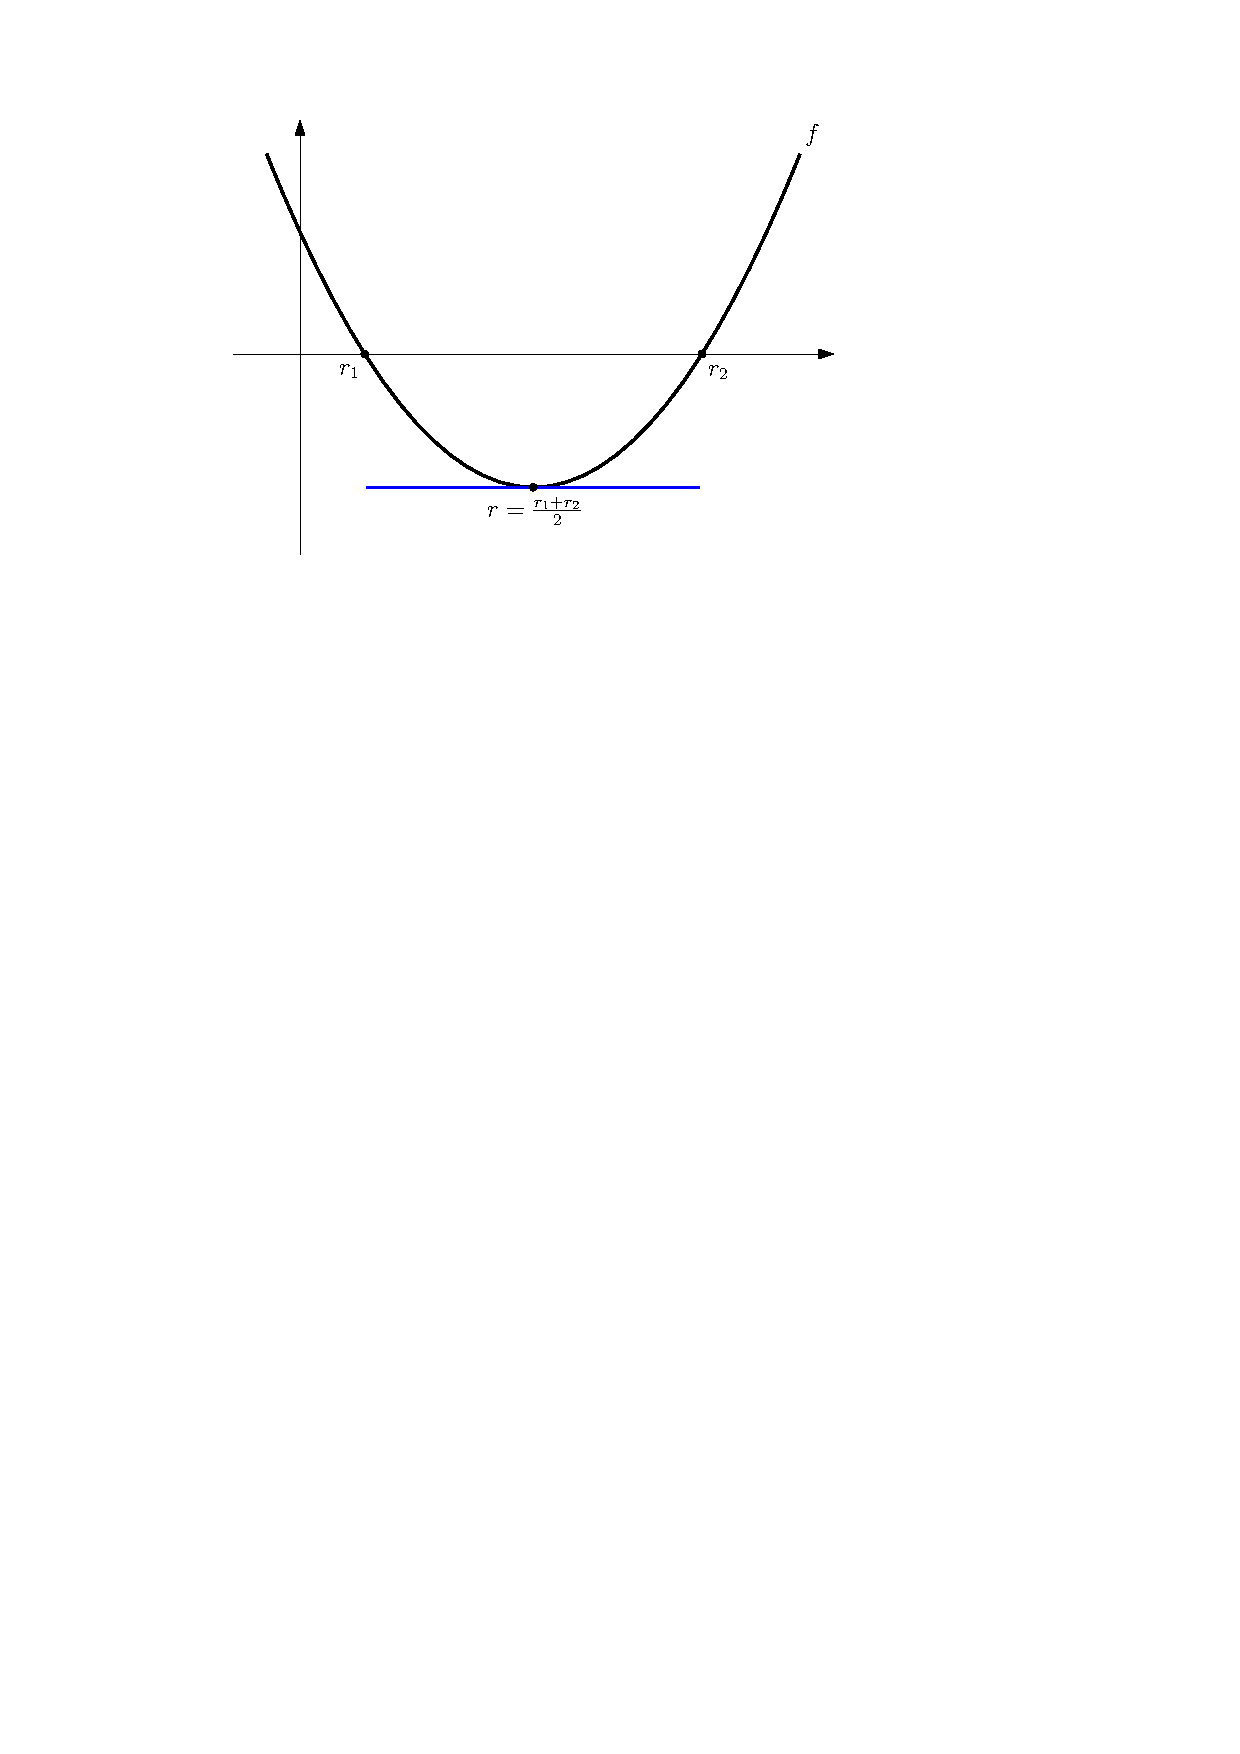
\includegraphics[scale=0.8]{polynomial_result}
\]
\begin{proof}[Proof of Proposition \ref{prop:highschool1}]
It is well-known that we may factor $f$ as follows:
\[
    f = a (x - r_1) (x - r_2) = a x^2 - a(r_1 + r_2) x + a r_1 r_2.
\]
Since two polynomials are equal if and only if their coefficients are equal we get $b = - a (r_1 + r_2)$, which gives us
\[
    \frac{df}{dx} (r) = 2 a r + b = 2 a \para{\frac{r_1 + r_2}{2}} - a (r_1 + r_2) = 0.
\]
This is the only solution since $\displaystyle\frac{df}{dx}$ is a first degree polynomial. Now note that $\displaystyle\frac{d^2 f}{d x^2}(x) = 2a \ne 0$ and $r_1 < r < r_2$ which gives us that
\[
    \text{sgn} \para{\frac{df}{dx}(r_1)} = -\text{sgn} \para{\frac{df}{dx}(r_2)} \ne 0.
\]
\end{proof}
When intersecting two of the paraboals of the beach line, we will find two intersection points, because of our assumptions. Proposition \ref{prop:highschool1} then gives us that at these intersection points $r_1, r_2$ we have that
\[
    \begin{cases}
        \displaystyle\frac{d(\beta_i - \beta_j)}{dx}(r_k) \ne 0 \text{ for } k = 1, 2 & \text{ }\vspace{0.25cm} \\ \text{sgn} \para{\displaystyle\frac{d(\beta_i - \beta_j)}{dx}(r_1)} = -\text{sgn} \para{\displaystyle\frac{d(\beta_i - \beta_j)}{dx}(r_2)} & \text{ }
    \end{cases}
\]
We then want to locate a specific breakpoint between two arcs, and the above will help us to do this.

To intersect the two parabolas $\beta_i$ and $\beta_j$ we write
\[
    (\beta_i - \beta_j)(x) = a x^2 + b x + c,
\]
where (for $p = p_i$, $q = p_j$, $h_p = p_y - \ell_y$ and $h_q = q_y - \ell_y$)
\begin{align*}
    a &= \frac{1}{2} \para{\frac{1}{h_p} - \frac{1}{h_q}}, \\
    b &= \frac{q_x}{h_q} - \frac{p_x}{h_p}, \\
    c &= \frac{q_y(p_x^2 + p_y^2) - p_y (q_x^2 + q_y^2) + \ell_y (q_x^2 + q_y^2 - p_x^2 - p_y^2) + \ell_y^2 (p_y - q_y)}{2 h_p h_q}.
\end{align*}
The square root of the discriminant is then
\[
    d = \sqrt{b^2 - 4 ac} = \sqrt{\frac{(p_x - q_x)^2 + (p_y - q_y)^2}{h_p h_q}}.
\]
The $x$-values of the intersection points are then given by the well-known formulas
\[
    r_1 = \frac{-b - d}{2 a}, \quad
    r_2 = \frac{-b + d}{2 a},
\]
which gives us the intersection points $q_1 = (r_1, \beta_i(r_1))$ and $q_2 = (r_2, \beta_i(r_2))$. Now, we want to find the breakpoint which at which an arc of $\beta_i$ exits the beach line, and an arc of $\beta_j$ enters the beach line. Proposition \ref{prop:highschool1} gives us a way of picking which one of $q_1$ and $q_2$ is the breakpoint that we need. For $\beta_i$ to exit and $\beta_j$ to enter, we need to pick $k$ such that
\[
    \frac{d \beta_i}{dx}(r_k) > \frac{d \beta_j}{dx}(r_k).
\]
This is illustrated in the following figure, with a slight abuse of notation:
\[
    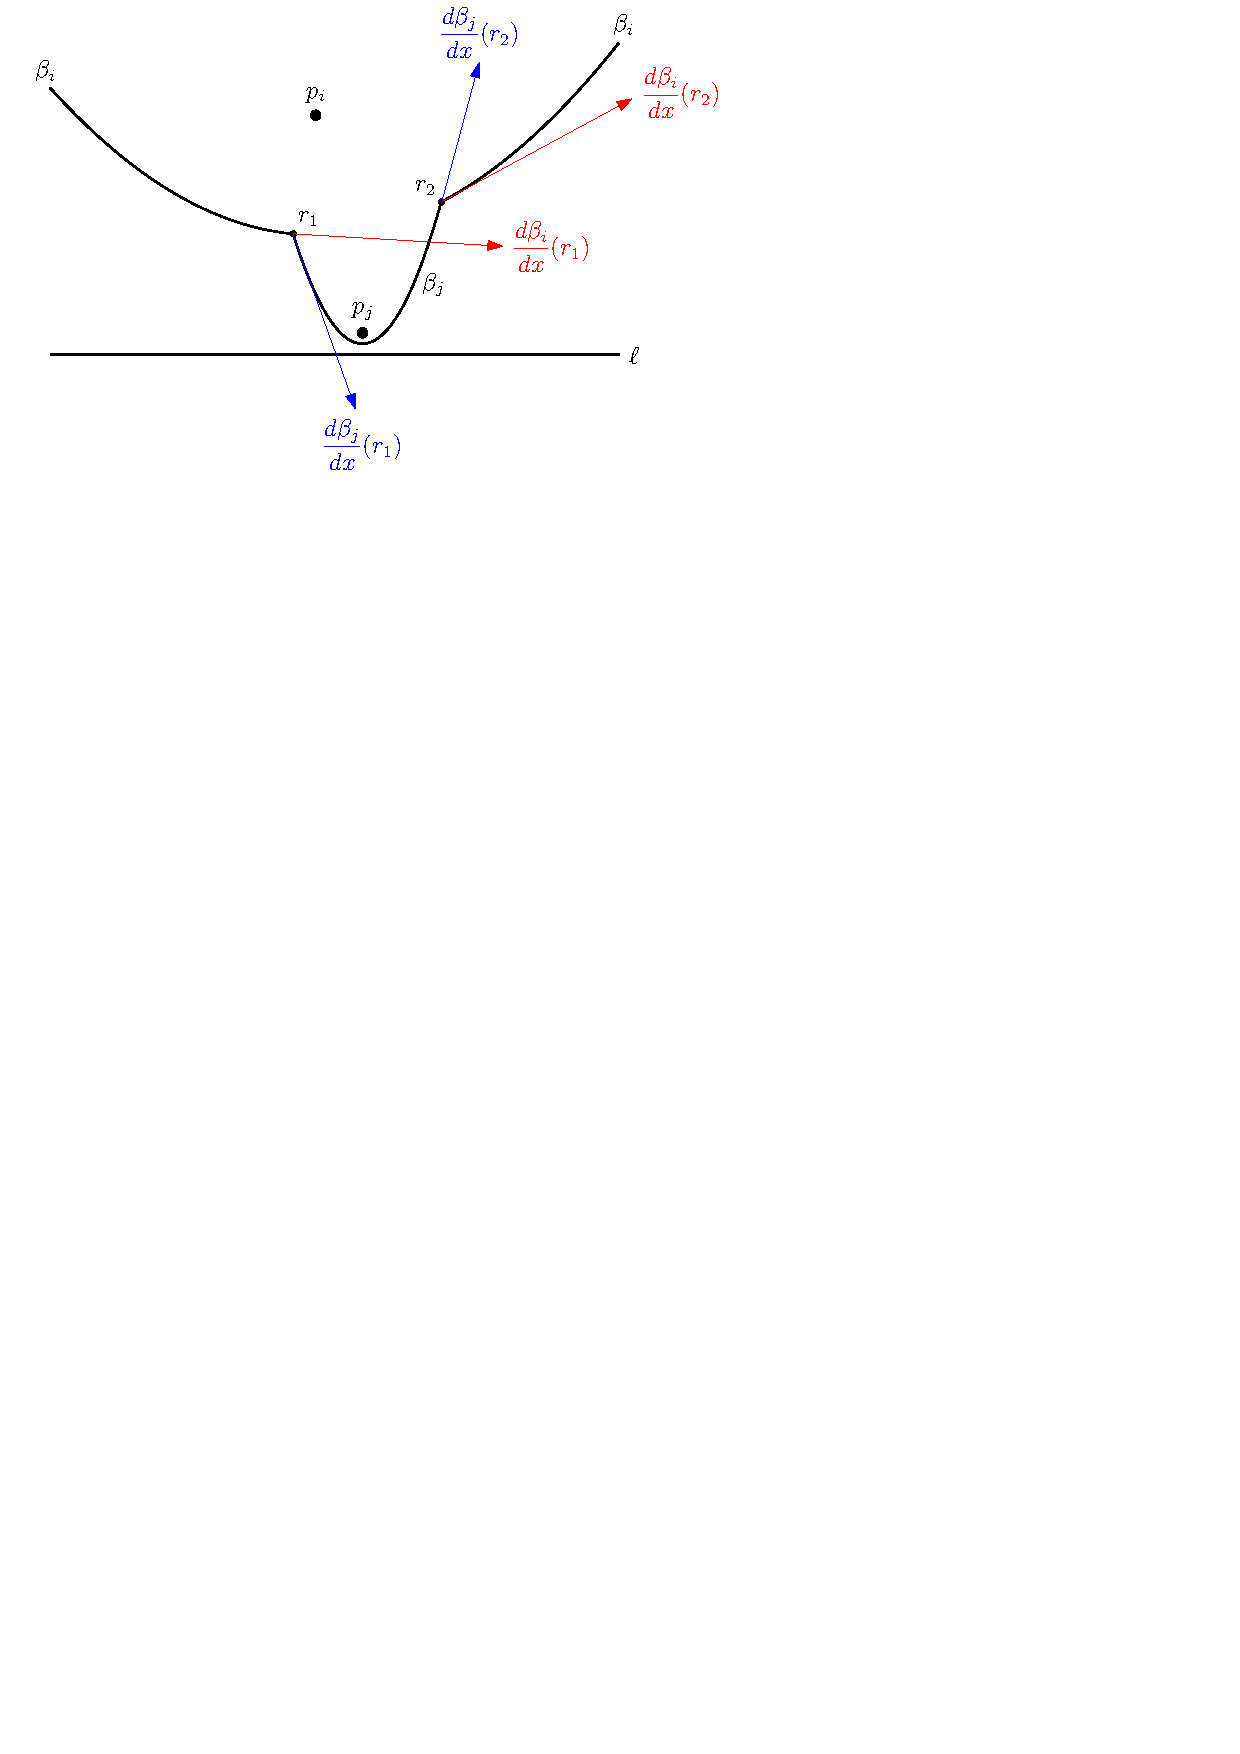
\includegraphics[scale=0.8]{derivativedirections}
\]
Proposition \ref{prop:highschool1} guarantees that either
\begin{align*}
    \frac{d \beta_i}{dx}(r_1) > \frac{d \beta_j}{dx}(r_1) &\text{ and } \frac{d \beta_i}{dx}(r_2) < \frac{d \beta_j}{dx}(r_2) \\
    &\text{or} \\
    \frac{d \beta_i}{dx}(r_1) < \frac{d \beta_j}{dx}(r_1) &\text{ and } \frac{d \beta_i}{dx}(r_2) > \frac{d \beta_j}{dx}(r_2),
\end{align*}
so it is possible to make the right choice. Now, note that by some simple algebraic manipulations we have that
\[
    \frac{d \beta_i}{dx}(r_k) > \frac{d \beta_j}{dx}(r_k)
\]
if and only if
\[
    (r_k - p_x) (q_y - \ell_y) > (r_k - q_x) (p_y - \ell_y).
\]
This gives us a criterion for deciding which intersection point describes the breakpoint in question, and this is the criterion used in the implementation.

\subsection*{Detail 3: How to find the arc vertically above a point}
At a site event when we discover a new point $p$ we want to find the arc $\alpha$ vertically above $p$, as illustrated here:
\[
    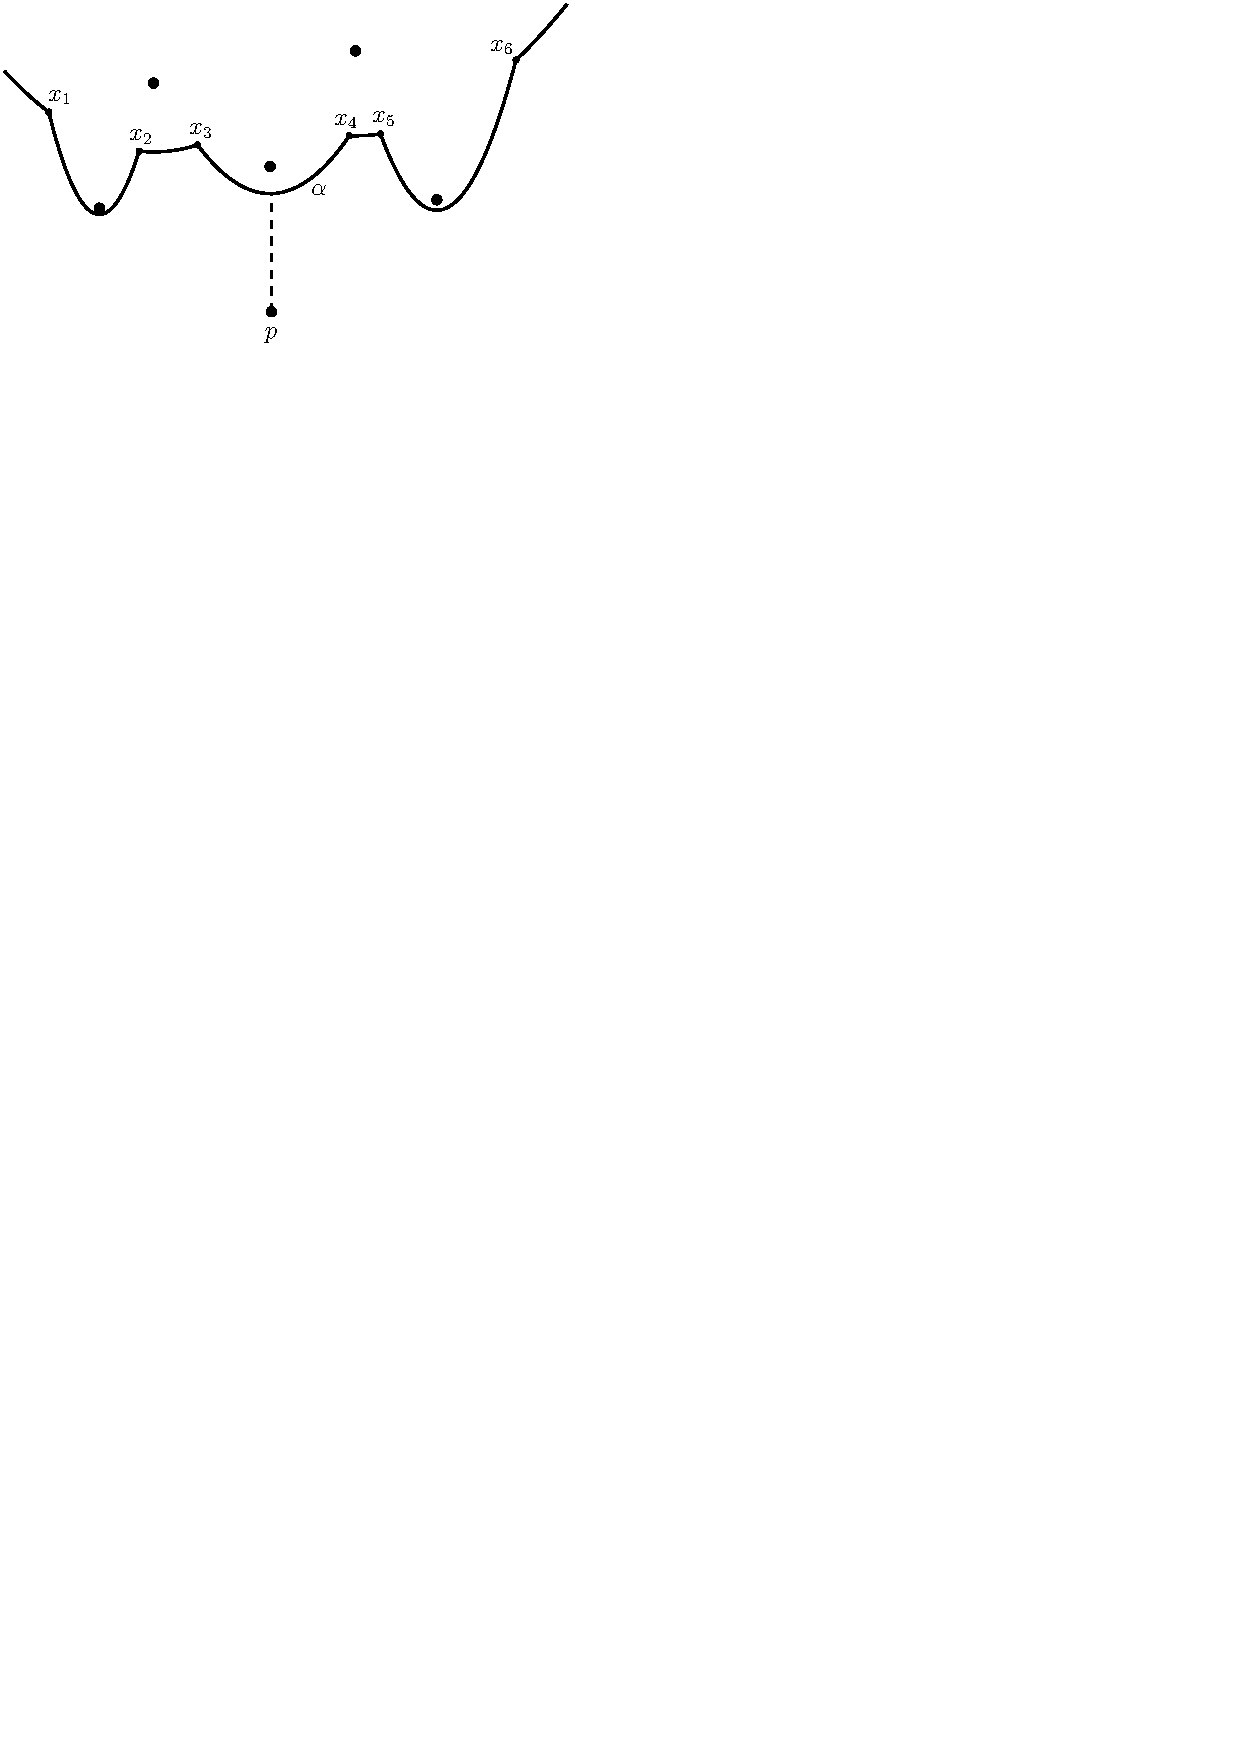
\includegraphics[scale=0.8]{locate_arc}
\]
Let $x_1, x_2, \ldots, x_k$ denote the breakpoints on the beach line. These are stored as internal nodes in our BST $\mathcal{T}$. Since the keys for the internal nodes are the $x$-values of the breakpoints, we may locate the arc $\alpha$ using binary search in $\mathcal{T}$. Starting at an internal node $x$ in $\mathcal{T}$ we visit its left subtree if $x\textsf{.key} < p_x$, and we visit its right subtree if $x\textsf{.key} \geq p_x$. The key property is computed at every check, since it is a function of the current position of the sweep line, see Detail 2 for how the key is computed. Eventually we will reach the leaf which stores the arc $\alpha$.

\subsection*{Detail 4: How to check if two breakpoints are converging}
Let $p, q, r$ be three sites from $P$ which define 3 consecutive arcs on the beach line. Let $x$ and $y$ be two breakpoints, where $x$ is sliding along $\bi(p, q)$ and $y$ is sliding along $\bi(q, r)$ as we vary $\ell$. We want to check whether $x$ and $y$ converge, and if so, what is the location of their intersection, and when during the sweep of $\ell$ will this occur. The two possible scenarios are illustrated below:
\begin{figure}[H]
    \centering
    \subfloat{
      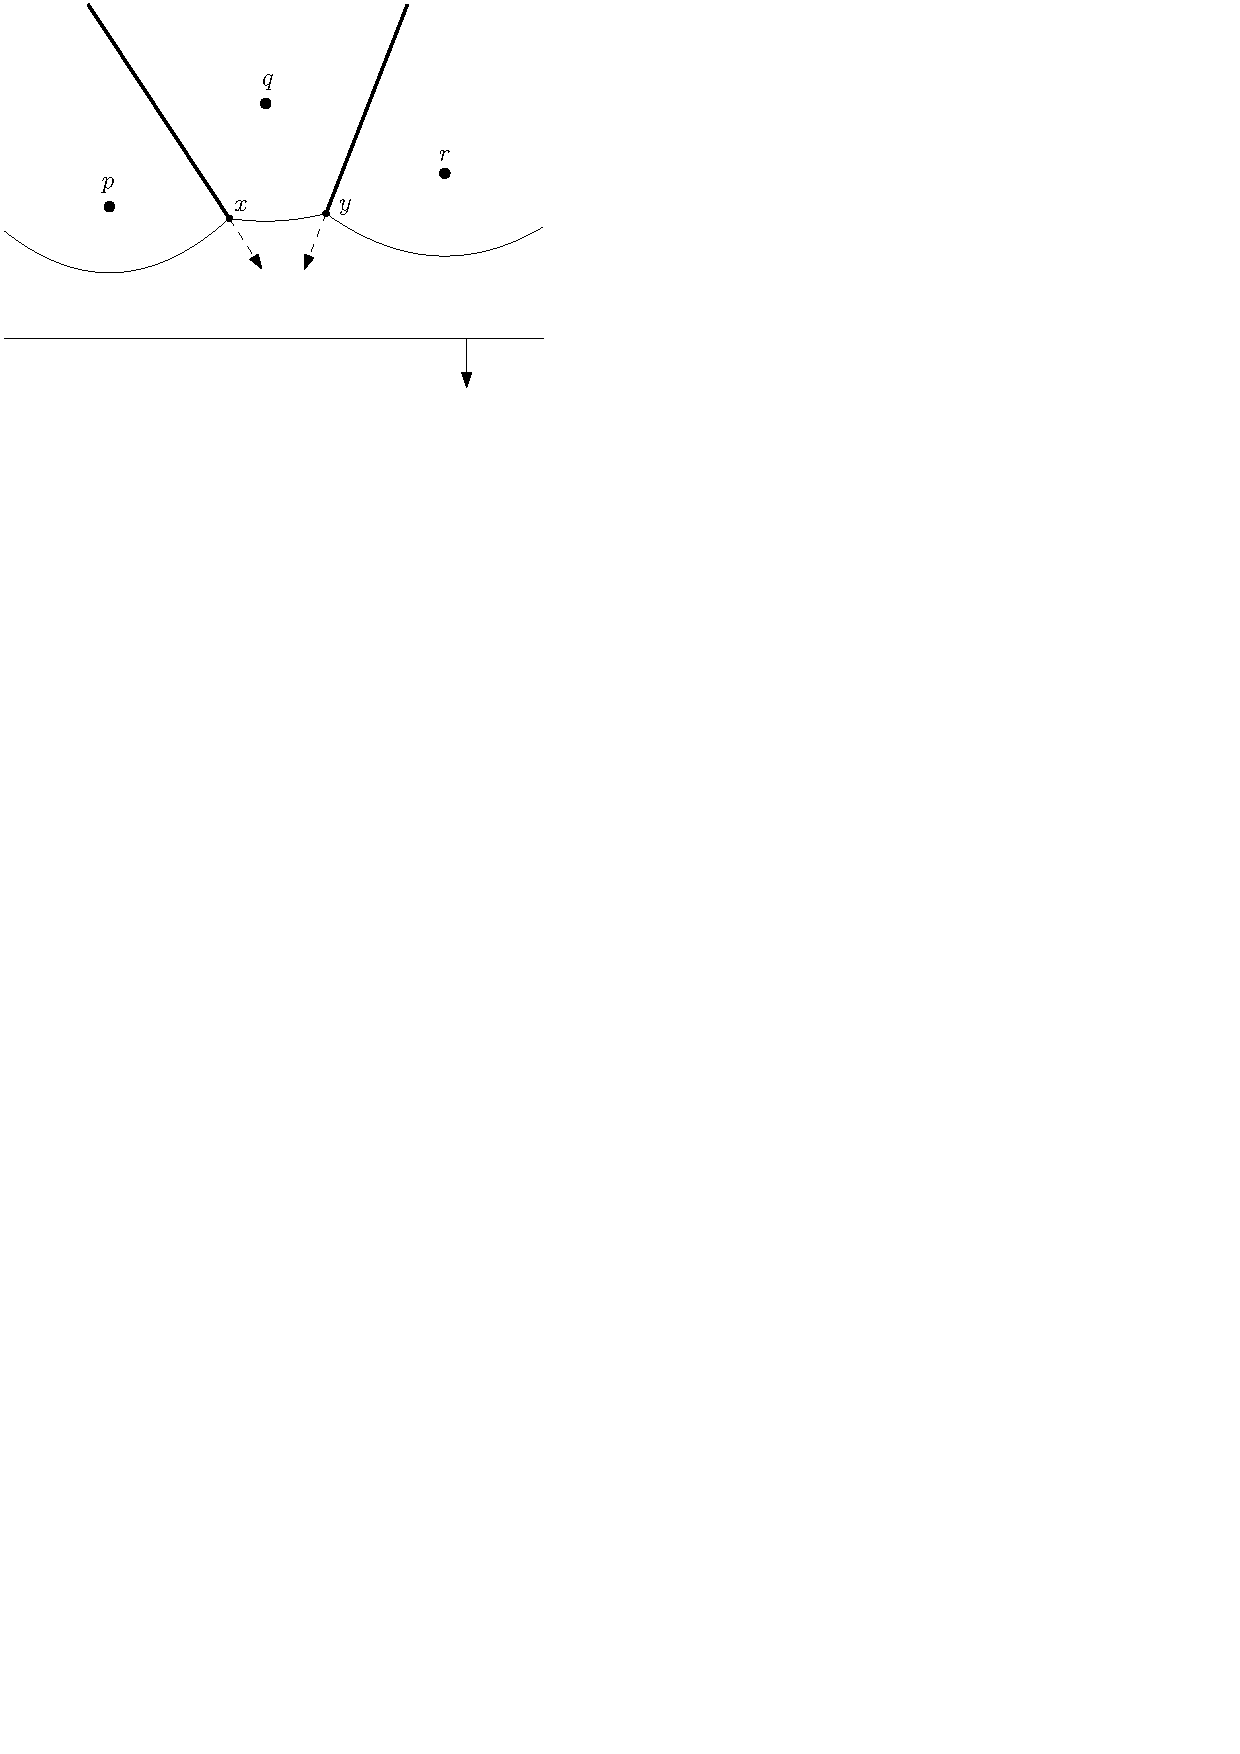
\includegraphics[scale=0.6]{converging_breakpoints_example}
    }
    \subfloat{
      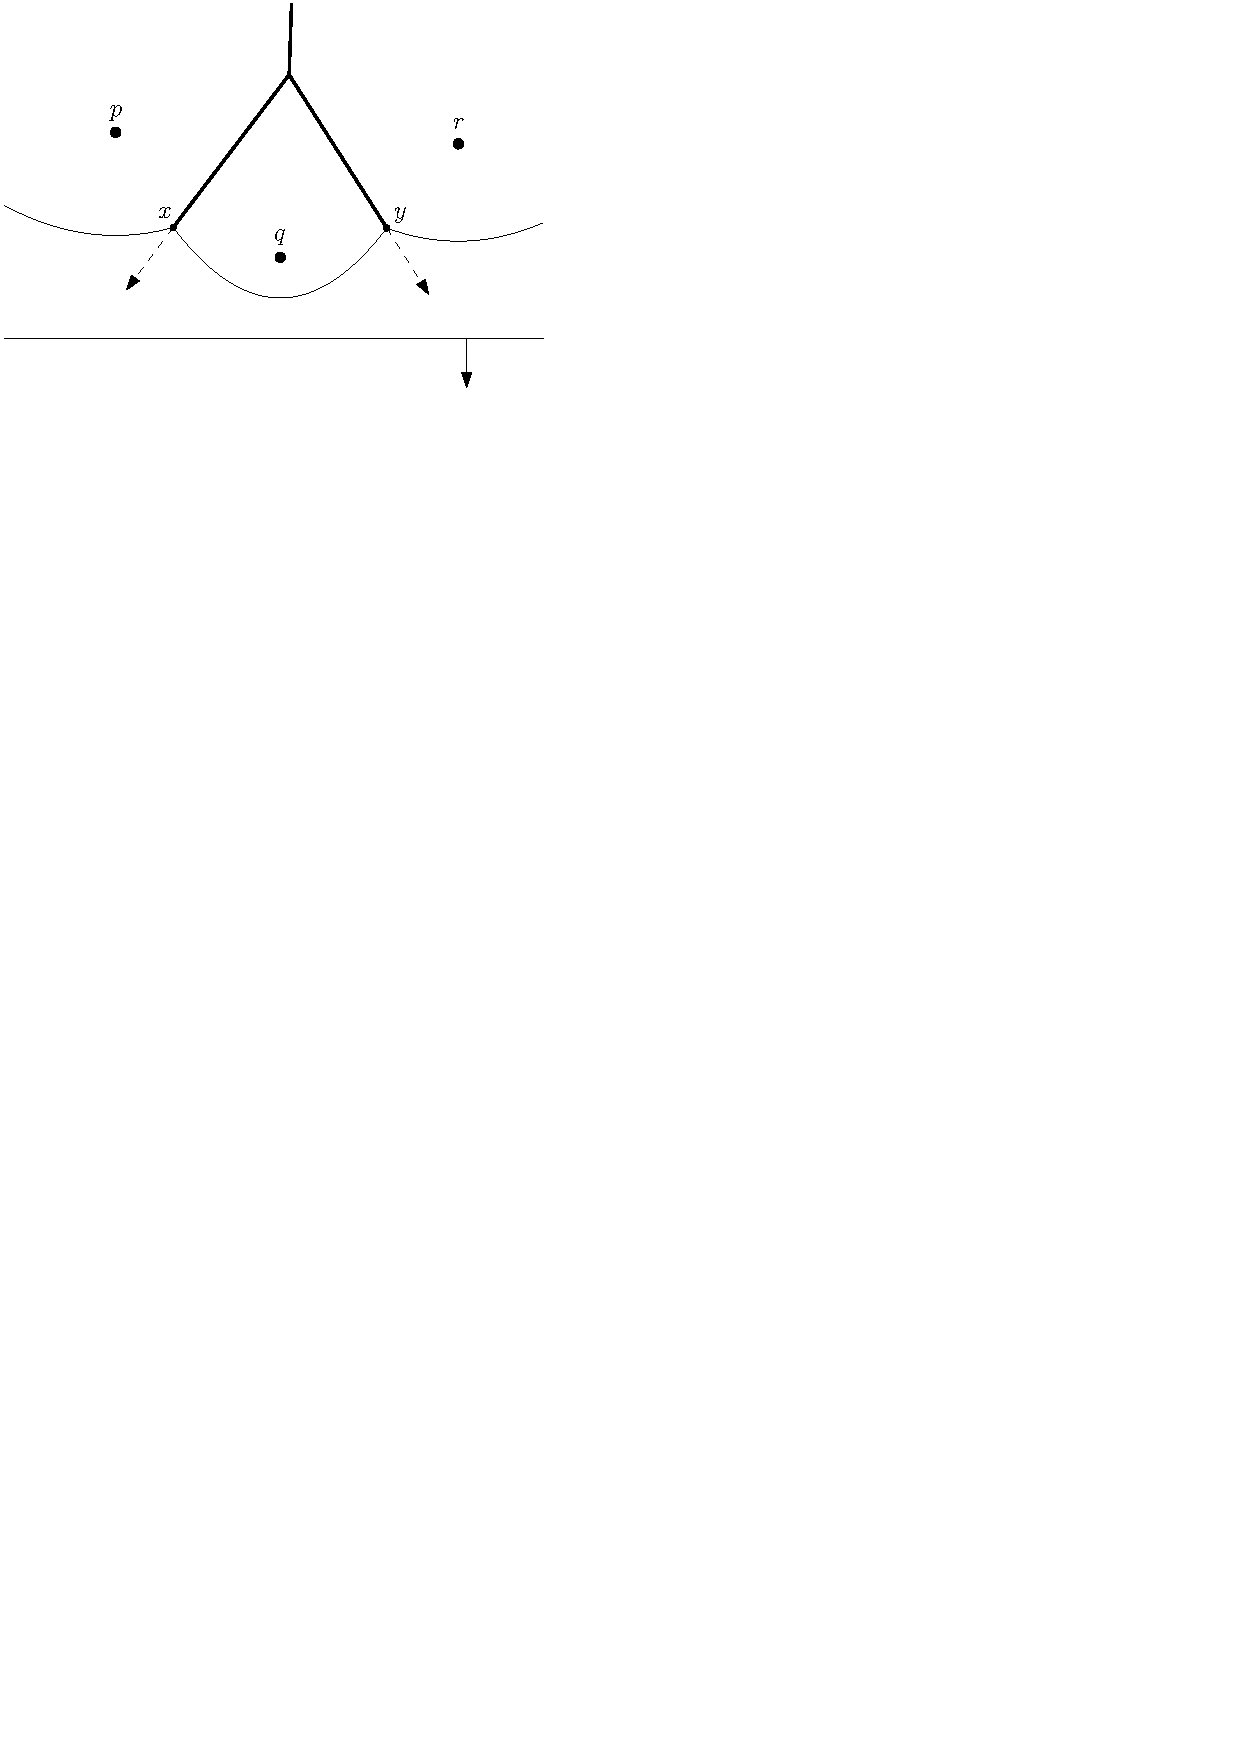
\includegraphics[scale=0.6]{converging_breakpoints_nonexample}
    }
\end{figure}
In the divergent case we include the case where the bisectors are collinear. 

To check for convergence, we transform the problem into a problem of intersecting two rays. Let $x$ and $y$ denote the current location of the breakpoints, and let $x'$ and $y'$ denote the breakpoints new positions after moving the sweep line some arbitrary amount downwards, and then let $d_1 = x' - x$ and $d_2 = y' - y$. Then $s \mapsto x + s d_1$ and $t \mapsto y + t d_2$ parametrize $\bi(p, q)$ and $\bi(q, r)$, respectively. The setup, in the case where the rays do intersect, looks like this:
\[
    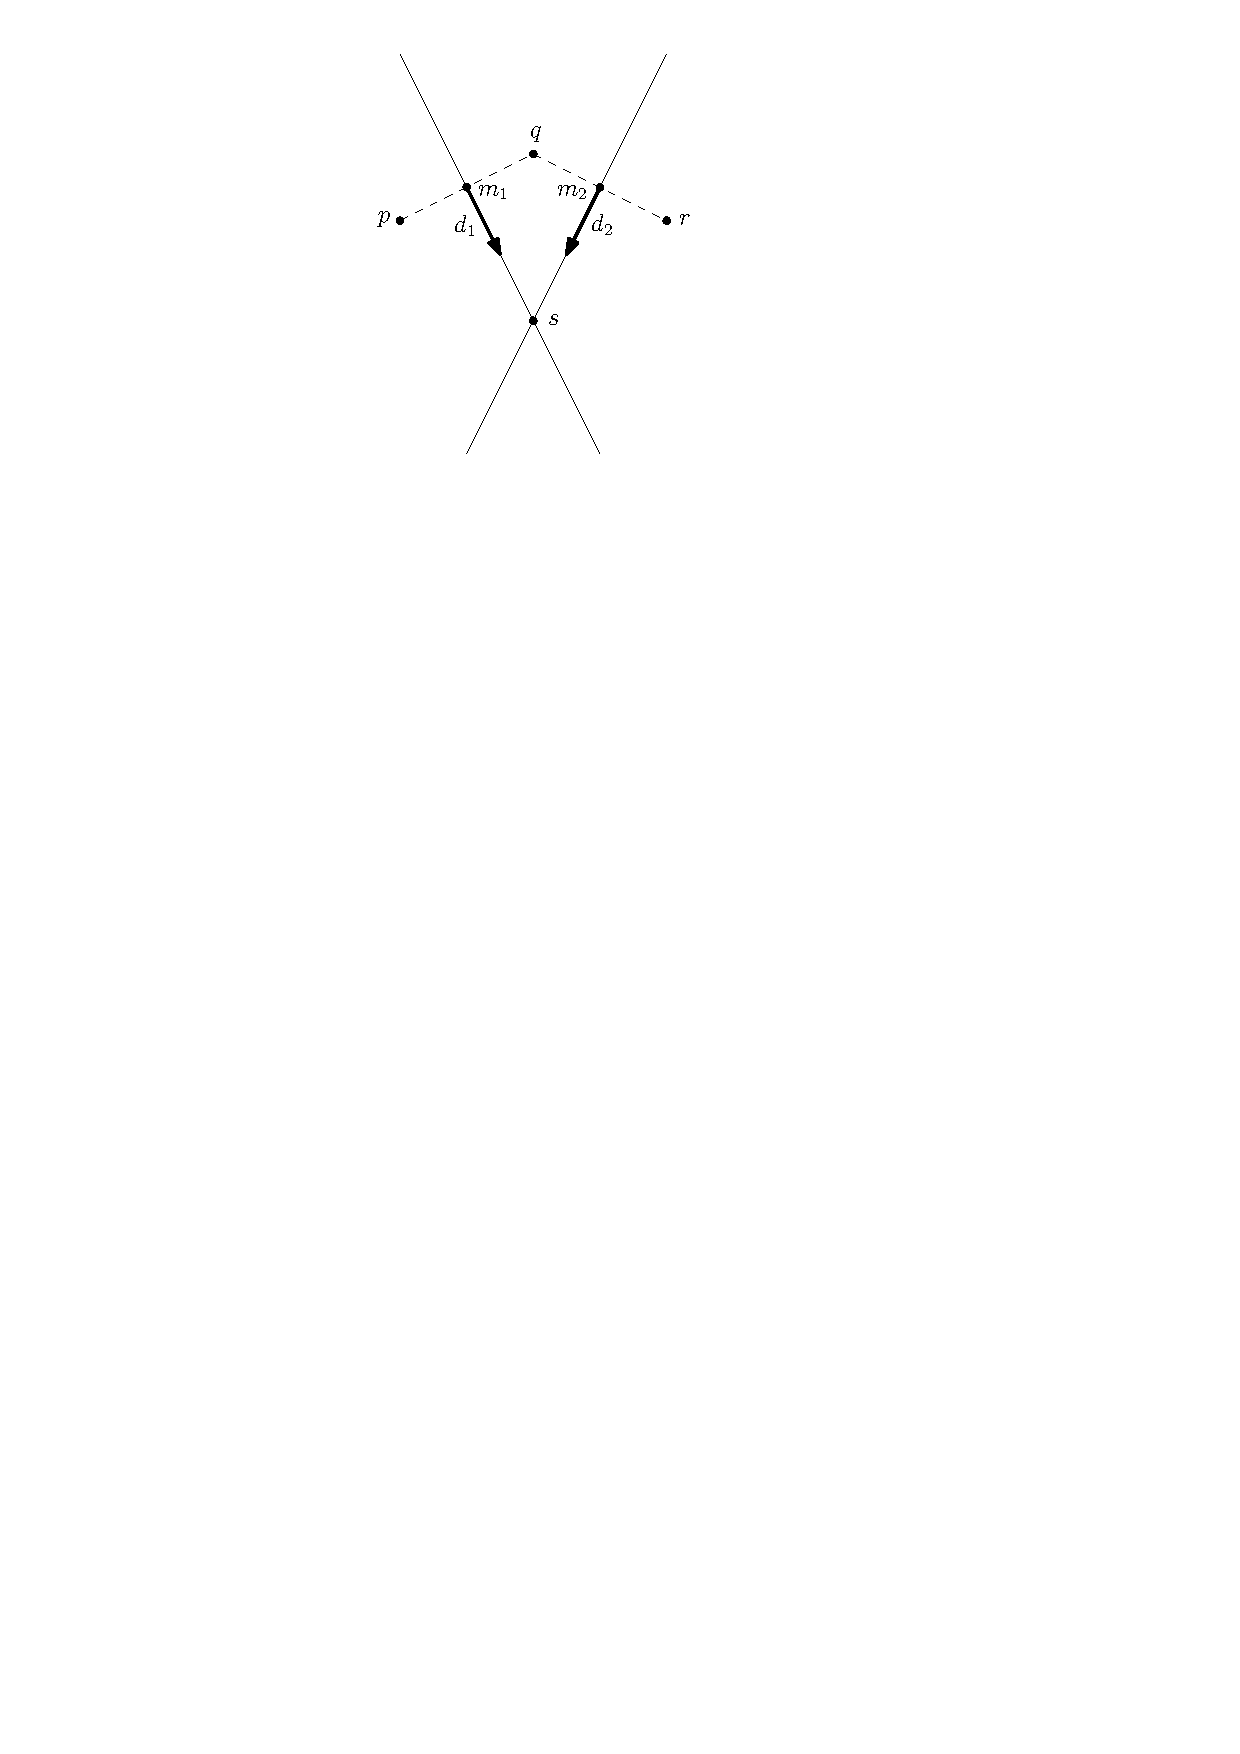
\includegraphics[scale=0.8]{ray_intersection}
\]
Now, as we saw in Detail 1, then the two rays converge if $t \geq 0$ and $s \geq 0$.

This can be interpreted as follows: If $s$ is positive, then that means that $x$ will hit $y$ in the future, and likewise if $t$ is positive, then $y$ will hit $x$ in the future. This is important as we are treating the events chronologically, and if $x$ and $y$ already intersected in the past (or the lines they describe, rather) then they can define no future circle event.

\subsection*{Detail 5: Finding a circle through 3 points}
As a part of the algorithm, we need to find the circle $C$ through 3 points $p, q, r$. It turns out if we intersect $\bi(p, q)$ and $\bi(q, r)$ we find the center of $C$, and then to find the radius we just need to find the distance from the center to one of the points. This is because if $x \in \bi(p, q) \cap \bi(q, r)$ then
\[
    \dist(x, p) = \dist(x, q) = \dist(x, r),
\]
so $x$ is exactly the center of a circle through $p, q, r$. This is illustrated in this figure:
\[
    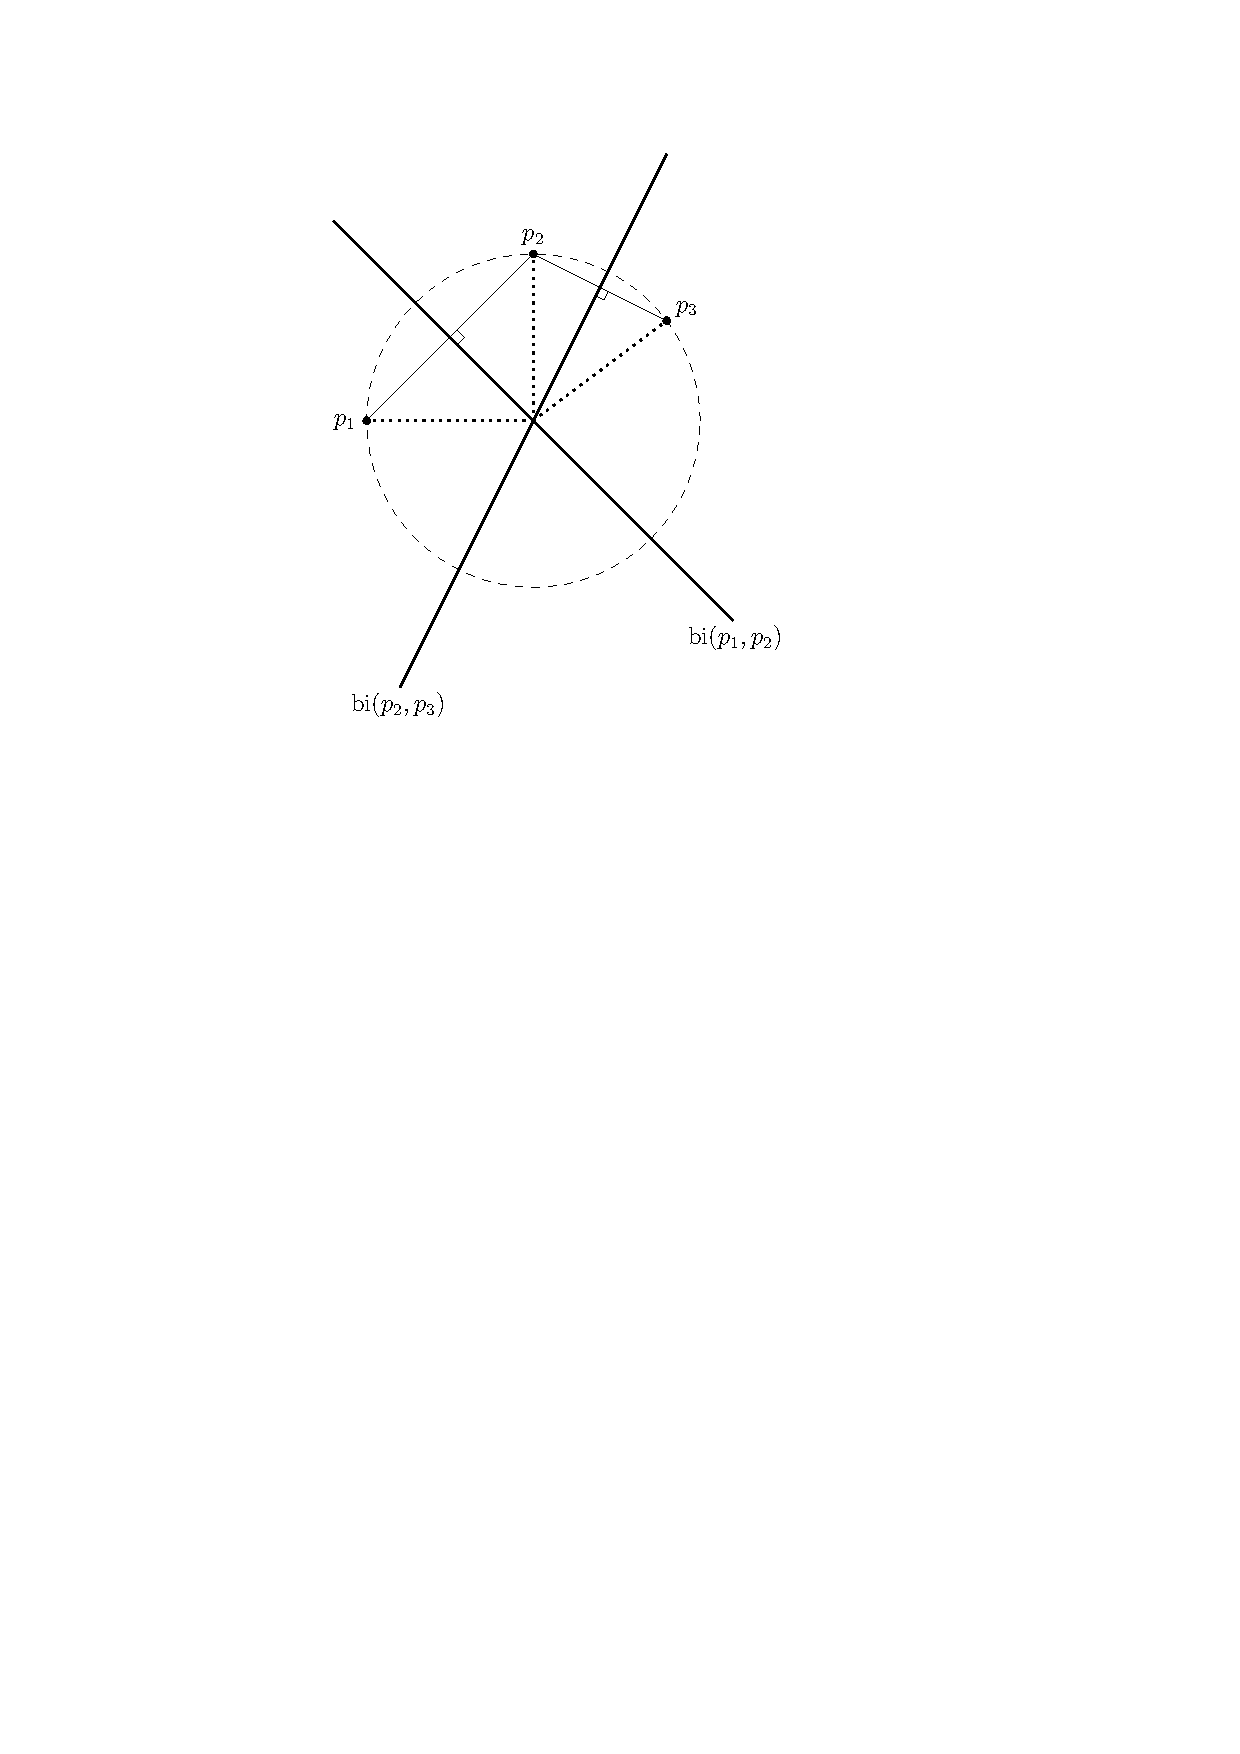
\includegraphics[scale=0.8]{circle_3_points}
\]
To intersect the bisectors, we form the midpoints
\[
    m_1 = \frac{1}{2}(p + q) \quad \text{and} \quad m_2 = \frac{1}{2}(q + r)
\]
and then we let $d_1$ and $d_2$ denote $q - p$ and $r - q$ rotated 90 degrees counterclockwise. Then $s \mapsto m_1 + s d_1$ and $t \mapsto m_2 + t d_2$ parametrize $\bi(p, q)$ and $\bi(q, r)$, respectively. Then we solve the linear system as in Detail 1.

\newpage
\subsection*{Detail 6: Deleting false alarms during a circle event}
At a circle event an arc disappears from the beach line, along with two breakpoints. Consider the following example, where at one point in time we have the arcs $\alpha_1, \alpha_2, \ldots, \alpha_7$ on the beach line along with the breakpoints $x$ and $y$ that $\alpha_5$ lies inbetween, and then after a circle event the arc $\alpha_5$ disappears after the breakpoints $x$ and $y$ intersect and get replaced by a new breakpoint $z$:
\[
    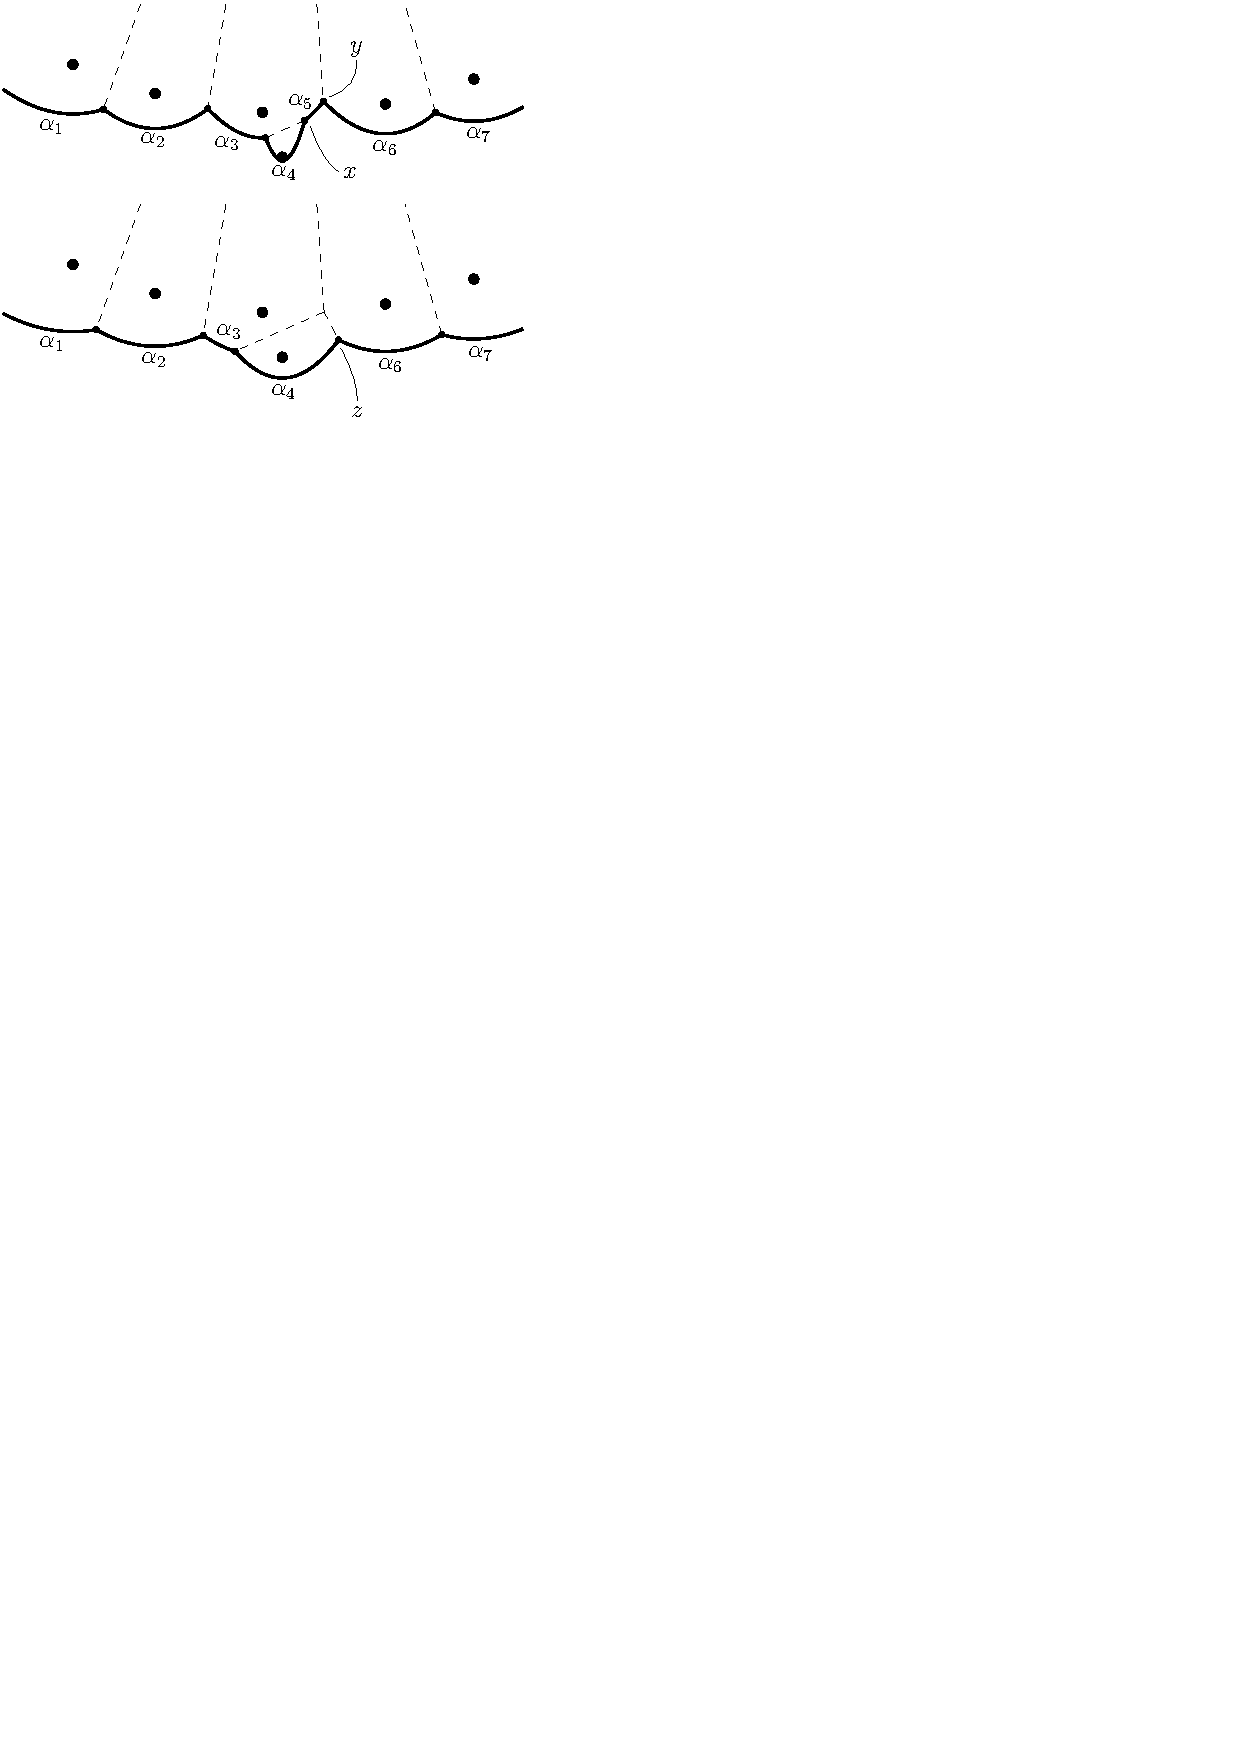
\includegraphics[scale=0.8]{circle_event_beachline_merge}
\]
When this happens, we have to remove the circle events that involve the breakpoints $x$ and $y$ merging with any other breakpoints. Since we set up a linked list of arcs, we can find the arcs $\alpha_4$ and $\alpha_6$ through the \textsf{.leftArc} and \textsf{.rightArc} pointers that $\alpha_5$ has, and if these arcs point to a circle event, then we remove those circle events from $\mathcal{Q}$ if they exist. This covers removing the false alarms, since we have removed circle events from every arc that surrounds $x$ and $y$. This example is general enough to explain the general case.

\subsection*{Detail 7: Intersecting a bounding box with the in-progress DCEL to get the final DCEL}

\section{Correctness}
\begin{lem}
Algorithm \ref{alg:fortune} can be implemented such that it runs in $\mathcal{O}(n \log n)$ time and uses $\mathcal{O}(n)$ storage.
\end{lem}
\begin{proof}
\todo{.}
\end{proof}